\documentclass[runningheads]{llncs}
% Grundgröße 12pt, zweiseitig
% Standardpakete
% richtiges encoding fuer verschiedene compiler
\usepackage{iftex}
\ifPDFTeX
   \usepackage[utf8]{inputenc}
   \usepackage[T1]{fontenc}
   \usepackage{lmodern}
\else
   \ifXeTeX
     \usepackage{fontspec}
   \else 
     \usepackage{luatextra}
   \fi
   \defaultfontfeatures{Ligatures=TeX}
\fi
% deutsche Silbentrennung
\usepackage[ngerman]{babel}
\usepackage{amsmath}
\usepackage{cite}
\usepackage{float}


% Grafiken einbinden
\usepackage{graphicx}
\graphicspath{{images/}}

\usepackage{hyperref}
% tiefe des Inhaltsverzeichnisses
\setcounter{tocdepth}{2}

\begin{document}

\title{Transaktionen}
\author{Ture Claußen, 1531067, \email{ture.claussen@stud.hs-hannover.de} \and Jannes Neemann, 1530893, \email{jannes.neemann@stud.hs-hannover.de}}
\authorrunning{T. Claußen \and J. Neemann}
\institute{Fakultät IV, Abteilung Informatik, Hochschule Hannover, Ricklinger Stadtweg 120, 30459 Hannover}

% jetzt gehts los
{\def\addcontentsline#1#2#3{}\maketitle} % Wird gebraucht, damit der Title nicht im Inhaltsverzeichnis steht

\begin{center} \sffamily\bfseries Selbständigkeitserklärung \end{center}
% fett und zentriert in der minipage

Mit der Abgabe der Ausarbeitung erklären wir, dass wir die eingereichte Seminar-Arbeit
selbständig und ohne fremde Hilfe verfasst, andere als die von uns angegebenen Quellen
und Hilfsmittel nicht benutzt und die den benutzten Werken wörtlich oder
inhaltlich entnommenen Stellen als solche kenntlich gemacht haben.
\vspace*{7ex}

Hannover, den \today \hfill

\begin{abstract}
  Eine explorative Betrachtung von Transaktionen in Ethereum. Erläuterung der technischen Spezifikationen, Untersuchung des aktuellen Zustands von Transaktionen und Erklärung eines Beispiels.

  \keywords{Ethereum \and Transaktionen \and RLP \and Gas \and Propagation}
\end{abstract}

\section{Einführung}
Das Wort Transaktion stammt von dem lateinischen Wort \textit{transigere} ab, welches im übertragenden Sinne mit "`durchführen"', "`vollführen"' oder "`abmachen"' (Geschäft) übersetzt werden kann. \cite{noauthor_transigere_nodate} Dieser Wortsinn besteht auch weiterhin im technischen und wirtschaftlichen Bereich, jedoch gibt es noch spezifischere Abgrenzungen. In der Wirtschaft ist es ein Vorgang bei dem Waren und Forderungen ausgetauscht werden. \cite[S. 18 f.]{ehrlicher_kompendium_1975} In der Informatik ist es im Zusammenhang mit Datenbanken eine unteilbare, \textit{atomare}, Abfolge von Anweisungen, die einen Übergang von einem konsistenten Zustand in einen Anderen beschreibt. \cite[S.520]{herold_grundlagen_2017}

Ethereum ist ein "transaktionsbasierter Automat" (\textit{transaction-based state machine}). Somit sind Transaktionen ein grundlegender Baustein von Ethereum im Allgemeinen und ihnen kommt eine ähnliche Bedeutung wie ACID Transaktionen bei. Der Automat speichert seinen Zuständ $ \sigma_t $ in der Blockchain, eine Transaktion $ T $ ist Argument der Zugstandsübergangsfunktion $ \Upsilon $, die von \textit{externen Akteuren (EA)} angestoßen wird und diesen gespeicherten Zustand $ \sigma_t $ in einen neuen, gültigen Zustand $ \sigma_{t + 1} $ überführen soll: $\sigma_{t+1} = \Upsilon(T, \sigma_t) $. Im Falle eines Konsens des Netzwerkes wird diese Zustandsveränderung durchgeführt beziehungsweise gespeichert.

Im Kontrast zu Kryptowährungen wie Bitcoin ist der Umfang des Automaten bzw. des Protokolls bei Ethereum deutlich geweitet, denn Zweck ist nicht nur die Schöpfung, Speicherung und der Austausch eines digitalen Zahlungsmittels \cite{nakamoto_bitcoin_nodate}, sondern eine allgemeine dezentrale Rechenmaschine, ein "Weltcomputer".  \cite[S. 1-4]{wood_ethereum/yellowpaper_2019} Im Folgenden betrachten wir eine beispielhafte Transaktion $ T_x $ von der Erzeugung, Signatur und Veröffentlichung, woran wir die technischen Spezifikationen von Transaktionen in Ethereum erläutern werden.

\section{Struktur und technische Umsetzung einer Transaktion}
Die Struktur einer Transaktion ist vergleichbar mit der eines Briefes. Es gibt jeweils einen Absender, Empfänger und eine Bezahlung für die Zustellungskosten. Bei Transkationen nicht in Form einer Briefmarke, sondern in Form von Gas (s. \ref{gas}). Außderdem kann beides eine "`Nutzlast"' \cite[S. 108]{antonopoulos_mastering_2019} enthalten. Dabei handelt es sich meistens um einenen Etherbetrag und/oder zusätzliche Daten. Genauso wie man in einem Brief Geld oder einen Text verschicken kann. Im Folgenden wird die allgemeine Struktur und technische Umsetzung von Transkation in Ethereum vorgestellt.

\subsection{Komponenten einer Transaktion}
\label{komponenten}
Transkationen, so auch unsere Transaktion $T_x$, enthalten laut ihrer offiziellen Definition \cite[S. 4]{wood_ethereum/yellowpaper_2019} folgende Datenfelder:
\begin{description}
  \item[nonce:] Ein Skalar welcher gleich der Anzahl der vom EOA versendeten Transaktionen ist. Der Nutzen wird in \ref{nonce} erläutert.
  \item[gasPrice:] Ein Skalar der angibt, wie viel Wei man pro Einheit \textit{Gas} bezahlt, die bei der Gesamtheit aller Berechnungen die während der Ausführung der Transaktion anfallen (s. \ref{gas})
  \item[gasLimit:] Ein Skalar der die maximal Anzahl an \textit{Gas} angibt, die während der Ausführung der Transaktion verbraucht werden darf. Dieser Betrag muss im Voraus bezahlt werden.
  \item[to:] Die 160-Bit Adresse des Empfängers.
  \item[value:] Skalar der die Menge Wei angibt, die der Empfänger erhält.
  \item[v,r,s:] Komponenten der ECDSA-Signatur (s. \ref{ecdsa}), um den Sender der Transaktion zu bestimmen
  \item[init:] Ein Byte-Array unbegrenzter Länge, welches nur bei einer Kontrakterzeugung verwendet wird und den kompilierten Sourcecode des Kontrakts enthält
  \item[data:] Ein Byte-Array unbegrenzter Länge, welches die Nutzdaten des Kontrakts enthält
\end{description}
Im Verlaufe dieser Ausarbeitung werden wir diese Felder für unsere Transaktion $T_x$ füllen und auf die genaue Bedeutung und auf weitere technische Spezifikationen dieser eingehen.


\subsection{Typen von Transaktionen}
\label{types}
Es gibt genau zwei Typen von Transaktion die in der Blockchain dokumentiert werden. Transaktionen die eine Nachricht von einem Account\footnote{Mit Account ist hier ein EOA oder ein Kontrakt gemeint} zu einem Anderem überträgt ("`message calls"' \cite[S. 4]{wood_ethereum/yellowpaper_2019}) oder Transaktionen die einen neuen Kontrakt erzeugen ("`contract creation"' \cite[S. 4]{wood_ethereum/yellowpaper_2019}). Mit Nachricht ist dabei der Inhalt von den Feldern \textit{value} und \textit{data} gemeint.

Bei Message-Call-Transaktionen enthält das \textit{to} Feld die öffentliche Adresse eines EOA oder eines Kontrakts. Unsere Transaktion $T_x$ adressiert einen Kontrak mit der Adresse \verb+0xd76595f64aaf9a79f27cf6831788f7575f0c7f38+. Zusätzlich besteht die Option die Felder \textit{value} und \textit{data} zufüllen. Speziell ist das \textit{data} Feld für unsere Transkation von Bedeutung. Denn der Funktionsaufruf wird in Bytecode in diesem gepeichert. Wie genau dies umgesetzt wird, ist in \ref{valData} genauer erläutert.

Die Besonderheit bei Contract-Creation-Transaktionen ist, dass die Empfängeradresse die Nulladresse (\textit{0x0}) ist. Diese Adresse ist keinem Account zugewiesen und dient ausschließlich als "`kontrakterzeugungs Adresse"' \cite{antonopoulos_mastering_2019}. Zusätzlich können Ether mitgesendet werden, die als Startfinanzierung des Kontrakt verwendet werden \cite[S. 4]{wood_ethereum/yellowpaper_2019}. Es sollten jedoch keine Ether an diese Adresse mit einer Message-Call-Transkation gesendet werden, da diese sonst verloren sind und nicht mehr zurückerstattet werden können \cite[S. 112]{antonopoulos_mastering_2019}.

Ein spezieller "`Typ"' von Transaktion ist eine interne Transaktion. Diese treten nur dann auf, wenn ein Kontrakt eine Transkation ausführt. Beispielsweise wird eine Funktion dieses Kontrakts aufgerufen und dem Sender ein Etherbetrag zurückgesendet. Die Transaktion mit dem Funktionsaufruf wird dabei in der Blockchain dokumentiert. Die Transkation mit der Überweisung aber nicht \cite[S. 40]{antonopoulos_mastering_2019}.

\subsubsection{Verteilung der Transaktionen}
Unter Betrachtung aller Transaktionen im Zeitraum vom 01.03.2020 00:00:17 UTC (Block 9581792) bis 31.03.2020 23:59:57 UTC (Block 9782601) mit dem Python Werkzeug \textit{ethereum-etl} \cite{noauthor_blockchain-etl/ethereum-etl_2020} und der API von \href{https://infura.io/}{\textit{infura}} lässt sich ein guter Eindruck von dem aktuellen Zustand des \textit{mainnets} von Ethereum gewinnen. Der Datensatz $ D $ enthält ein Gesamtvolumen $ M $ an 22,748,700 Transaktionen, wovon ~2.1\% Kontrakterzeugungen sind. Wiederrum sind X\% der Transaktionen an Kontrakte addressiert. Wir definieren den Gesamtwert einer Transaktion als $ V_{\text{total}} = \textit{gasPrice} \times \textit{gasLimit} + \textit{value} $, wobei wir diesen Wert der Empfängeraddresse zuschreiben. Ordnet man die Addressen nach $ V_{\text{total}} $ machen der kumulierte Wert $ \text{SUM}(V_{\text{total}}) $ der ersten 100 Addressen ~2.3\% des Gesamtwertes aus. Alle diese Adressen sind Kontrakte. Allerdings ist die Anzahl der Transaktion, die an diese Konktrakte addressiert sind, ~44.2\% des gesamten Transaktionsvolumens $ M $. \cite{neemann_appendix_nodate}

\subsection{Serialisierung}
Da Ethereum ein Weltcomputer ist, müssen Daten schnell, kompakt, effizient und einheitlich verschickt werden. Dabei wird das Kodierungsverfahren \textit{Recursive Length Prefix (RLP)} verwendet \cite[S. 100]{antonopoulos_mastering_2019}. Alle serialisierten Daten in Ethereum sind Listen von Bytes \cite[S. 3]{wood_ethereum/yellowpaper_2019}. Auch die Daten unserer Transaktion $T_x$ werden mit Hilfe von RLP in eine Liste von Bytes serialisiert und wieder deserialisiert. Bei der RLP Kodierung handelt es sich nur um ein Verfahren um Struktur zu serialisieren. Das heißt die Methode nimmt nur ein so genanntes "`Item"' als Parameter entgegen. Dieses Item ist entweder ein String, welcher in ein Byte-Array konvertiert wird, oder eine Liste von Items. Relevant ist für die Methode nur die Länge des Items. Je nach Fall werden dabei unterschiedliche Regeln definiert:
\begin{enumerate}
  \item Item ist eine Zeichenkette (Byte-Array):
        \begin{itemize}
          \item Besteht dieses nur aus einem Byte mit einem Wert kleiner als 128 (\texttt{0x7f}), ist das Byte ihre eigene RLP Repräsentation
          \item Enthält das Byte-Array weniger als 56 Byte, ist die RLP Repräsentation der Inhalt dieses mit einem Präfix von \texttt{0x80} (128) plus die Länge des Arrays. Beispiel: "`Ethereum"':
                \begin{center}
                  \texttt{[0x88, 'E', 't', 'h', 'e', 'r', 'e', 'u', 'm']}\\
                  bzw inkl. ASCII-Kodierung\\
                  \texttt{[0x85, 0x45, 0x74, 0x65, 0x68, 0x72, 0x65, 0x75, 0x6d]}
                \end{center}
          \item Ist das Byte-Array größer als 55 Byte wird ein Präfix aus mehreren Bestandteilen verwendet. Zum einen \texttt{0xb7} plus die Anzahl der Bytes die benötigt werden, um die Länge des String darzustellen. Gefolgt von der Länge des Strings im Big-Endian Format und dem Inhalt des Byte-Arrays. So ergibt sich für ein 2048-Byte langes Byte-Array folgender Präfix: \texttt{[0xb9, 0x80, 0x00]}.
                2048 entsprechen in Hexadezimal \texttt{0x800} somit werden zwei Bytes (\texttt{0x80} und \texttt{0x00}) benötigt, um die Länge des Bytes darzustellen. Somit erhalten wir $\texttt{0xb7} + 2 = \texttt{0xb9}$.
        \end{itemize}
  \item Item ist eine (verschachtelte) Liste von Items:
        \begin{itemize}
          \item Ist die Gesamtlänge aller in der Liste enthaltenen Items mit ihrer jeweiligen RLP Repräsentation 0-55 Bytes lang, so wird der Präfix \texttt{0xc0} plus die Länge der konkatenierten Liste der RLP Repräsentation gesetzt. Anschließend folgt die Liste selbst. So wäre die Kodierung der Liste \texttt{["`Ether"', "`Wei"']}:
                \begin{center}
                  \texttt{[0xca, 0x85, 'E', 't', 'h', 'e', 'r', 0x83, 'W', 'e', 'i']}\\
                  bzw. inkl. ASCII-Kodierung\\
                  \texttt{[0xca, 0x85, 0x45, 0x74, 0x68, 0x65, 0x72, 0x83, 0x57, 0x65, 0x69]}
                \end{center}
                Das zweite bis siebte Byte ist dabei die RLP Repräsentation von "`Ether"' und die Bytes acht bis elf die von "`Wei"'. Somit ergibt sich eine Länge von 10 Byte und der Präfix \verb+0xca+.
          \item Ab einer Gesamtlänge von 56 Bytes wird der Präfix \texttt{0x7f} plus die Anzahl der Bytes die benötigt werden, um die Länge der Liste darzustellen. Danach folgt die Länge der Liste mit der konkatenierten Liste von RLP Repräsentation
        \end{itemize}
\end{enumerate}
Das Item darf nicht länger als $2^{64}$ Bytes sein, da sonst die Länge des Präfix in allen Fällen länger als 255 ist und somit nicht in einem Byte dargestellt werden kann \cite[S.18,19]{wood_ethereum/yellowpaper_2019}.
\section{Aufbau einer Transaktion}

\subsection{Nonce}
\label{nonce}
Die Nonce wurde nicht von Ethereum eingeführt, sondern kommt aus dem Bereich der Kryptographie. Eine Nonce ist dort laut Definition \cite{noauthor_ethereum/wiki/rlp_nodate}
eine willkürliche Nummer, die nur einmal in einer kryptographischen Kommunikation verwendet wird. Dabei handelt es sich meistens um eine zufällig oder pseudo-zufällig generierte Zahl. Mit der die Einmaligkeit der Kommunikation gesichert wird.

In Ethereum-Transaktionen ist die Nonce eine Zahl, welche bei der Accounterstellung den Wert Null hat und bei jeder erfolgreichen Transaktion\footnote{Eine Transaktion ist erfolgreich, wenn sie in einem Block der Blockchain aufgenommen wurde} um eins inkrementiert wird. Dieser Wert wird dabei nicht explizit im Account gespeichert, sondern dynamisch die Anzahl der erfolgreichen Transkationen wird gespeichert \cite[S.101]{antonopoulos_mastering_2019}.

Mit der Nonce werden sogenannte "Replay attacks" verhindert. Im Rahmen von Ethereum gesprochen wird so verhindert, dass die selbe Transkation mehrmals ausgeführt werden kann. Da Transaktionen in der Blockchain gespeichert werden und alle Daten zu dieser Transkation eingesehen werden können, wäre es ohne die Nonce möglich, dass ein Unbeteiligter der Transkation diese unbegrenzt oft wiederholen kann, ohne die Zustimmung des Absenders zu haben. Da die Transkation jedoch schon einmal abgeschlossen ist, entsprechen die Noncen des Absenders und der Transkation nicht mehr überein, somit wird die Transaktion abgelehnt. Auch der eigentliche Absender selbst, kann diese Transaktion demnach nicht mehr wiederholen.

Des Weiteren dient die Nonce auch der Transaktionsabwicklung innerhalb des Netzwerks.  Werden mehrere Transaktionen von einem Account versendet, kommen diese meistens in unterschiedlicher Reihenfolge bei den Nodes an. So ist nicht sichergestellt, dass eine Transaktion die eine höhere Priorität hat, auch als erste verarbeitet wird. Mit der Nonce kann dies jedoch realisiert werden. So vergleicht das Netzwerk die Nonce, die mit der Transkation gesendet wird, mit der Nonce des Account. Stimmen diese überein, so wird die Transkation sofort verarbeitet. Ist die Nonce der Transaktion größer als die erwartet, landet die Transkation im \textit{Mempool}, in dem sich alle noch nicht verarbeiteten Transkationen befinden. Ist die Nonce des Accounts zum Beispiel 2 und die der Transkation 5, so geht der Node davon aus, dass die Transaktionen mit den noch fehlenden Noncen sich verspäten. Somit bleibt die Transaktion solange im Pool, bis die Transaktion mit den Nonce 2, 3 und 4 im Netzwerk registriert wurden. Somit kann eine Priorisierung von Transaktionen durch eine in der Priorität absteigende Transaktionsreihenfolge sichergestellt werden.

\subsection{Value und Data}
\label{valData}
Wie in \ref{komponenten} schon vorgestellt, enthalten das \textit{value}- und \textit{data}-Feld die eigentliche Nutzlast einer Transaktion. Dabei enthält das \textit{value}-Feld ausschließlich den Betrag an Wei, der an die Empfängeradresse gesendet werden soll und das \textit{data}-Feld enthält die Nachricht.
Eine Transkation, die ein \textit{value}-Feld enthält, wird dabei auch Zahlung bzw. \textit{payment} genannt. Das \textit{data}-Feld ist ein Aufruf bzw. \textit{invocation}\cite[S.108]{antonopoulos_mastering_2019}. Eine Zahlung zwischen zwei EOAs ist dabei eine einfache Zustandsänderung der EVM und Übertragung des Etherbetrags in Weis auf den empfangenden Account. Enthält diese Transkation Daten im \textit{data}-Feld, so wird diese von der Blockchain ignoriert \cite[S.10]{wood_ethereum/yellowpaper_2019}. So werden diese auch von der eigenen Wallet ignoriert und nur angezeigt.
\begin{figure}[h!]
  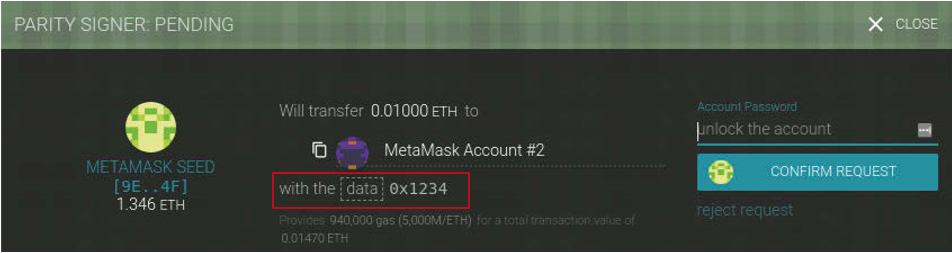
\includegraphics[width=\textwidth, keepaspectratio]{dataTransaction.png}
  \caption{Beispieltranskation an EOA mit gefülltem \textit{data}-Feld \cite[S.109]{antonopoulos_mastering_2019}}
\end{figure}

Wie bereits in \ref{types} erwähnt, wird der Inhalt des \textit{data}-Feld erst von Interesse, wenn wir einen Kontrakt ansprechen.
Beispielsweise soll unsere Transkation die Funktion \\
\begin{verbatim}
  function deposit(string _depositReason) public payable {
    balances[msg.sender] += msg.value;
    reasons[msg.sender].push(_depositReason);
  }
\end{verbatim}
des Kontrakts aufrufen. Diese Funktion fügt den kontraktinternen Konto dem im \textit{value}-Feld übergeben Wert hinzu. Dabei muss als Parameter der Einzahlungsgrund genannt werden.

Damit diese Funktion aufgerufen werden kann, muss der Funktionsaufruf der Spezifikation des \textit{Contract Application Binary Interface (ABI)} entsprechen \cite{noauthor_contract_nodate}.
Das heißt, der endgültige Inhalt setzt sich im allgemeinen aus dem Funktionsselektor und den Funktionsargumenten zusammen. Der Funktionsselektor teilt dem Kontrakt mit, welche Funktion er ausführen soll und entspricht den ersten vier Bytes des Keccak-256-Hash des Funktionsprototypen. Keccak-256 ist das am meisten verwendete Hashverfahren in Ethereum \cite[S. 3]{wood_ethereum/yellowpaper_2019}. Laut ABI Spezifikation setzt sich der Funktionsprototyp aus dem Namen der Funktion und in Klammern folgend die einzelnen Parametertypen. Der Rückgabetyp einer Funktion ist nicht Teil des Funktionsprototyps.

Daraus resultiert folgender Prototyp für unsere Funktion: \verb+deposit(string)+.
Dessen vollständiger Keccak256-Hash entspricht:
\begingroup
\fontsize{8pt}{10pt}\selectfont
\begin{center}
  \verb+0xa26e11860cdb80ecca46e4f433c3c9533f6d37cdf0f6eb16343556cfdbcf47ec+
\end{center}
\endgroup
Somit entspricht \verb+0xa26e1186+ dem ABI konformen Funktionsselektor.\\
Unser Funktionsaufruf soll $1000000000000000000$ Wei (entspricht einem Ether) auf das Konto einzahlen. Als Parameter übergeben wir "`Einzahlung"'. Um einen String ABI konform zu kodieren, müssen wir den Offset angeben, ab dem der Inhalt unseres Parameters startet, konkatiniert mit der Länge des Strings und beides nach links auf 32 Byte mit Paddingsbytes aufgefüllt. Danach folgt der String in UTF-8 kodiert, welcher nach rechts auf 32 Bytes aufgefüllt wurde. In unserem Fall müssen wir 32 Zeichen überspringen (\texttt{0x20}). Der String ist 10 (\texttt{0xa}) Zeichen lang. Somit lautet die Kodierung unserer Funktionsargumente wie folgt:
\begingroup
\fontsize{8pt}{10pt}\selectfont
\begin{center}
  \texttt{0x0000000000000000000000000000000000000000000000000000000000000020 \textbackslash} \\
  \texttt{000000000000000000000000000000000000000000000000000000000000000a \textbackslash} \\
  \texttt{45696e7a61686c756e6700000000000000000000000000000000000000000000}
\end{center}
\endgroup
Unsere Nutzlast, welche wir im \textit{data}-Feld nun eintragen müssen, erhalten wir aus der Konkatenation beider Kodierungen:
\begingroup
\fontsize{8pt}{10pt}\selectfont
\begin{center}
  \texttt{0xa26e1186 \textbackslash} \\
  \texttt{0000000000000000000000000000000000000000000000000000000000000020 \textbackslash} \\
  \texttt{000000000000000000000000000000000000000000000000000000000000000a \textbackslash} \\
  \texttt{45696e7a61686c756e6700000000000000000000000000000000000000000000}
\end{center}
\endgroup
Man kann jedoch über das \textit{data}-Feld keinen Ether an den Kontrakt übergeben. Dies ist ausschließlich über das \textit{value}-Feld möglich. Damit der Kontrakt dieses Ether annimmt, muss die Funktion genau wie unsere Funktion mit dem Schlüsselwort \texttt{payable} deklariert sein. Akzeptiert die aufgerufene Funkntion kein Ether, so wird die sogenannte Fallback-Funktion aufgerufen, die den übergenenen Etherbetrag auf das Konto des Kontrakts gutschreibt. Ist auch diese nicht definiert, wird eine Exception geworfen und die Transaktion abgebrochen \cite{noauthor_contract_nodate}.

Die letzte mögliche Kombination ist, wenn sowohl das \textit{value}- und \textit{data}-Feld leer sind. Dies ist ebenfalls eine gültige Transkation. Diese erfüllt jedoch keinen besonderen Zweck, außer der Verwendung des bezahlten Gas und somit nur einer Senkung des eigenen Kontostands.

\subsection{Gas}
\label{gas}
Gas ist ein zentraler konzeptioneller Lösungsansatz im Rahmen von Ethereum. Da Ethereum turing-vollständig ist \cite[S. 1]{wood_ethereum/yellowpaper_2019}, ergibt sich unter anderem das sogenannte "`Halteproblem"'. Dieses besagt, dass im Voraus nicht vorhergesagt werden kann, ob das Programm einer Turing-Maschine jemals zu einem Ende kommt. \cite[S.70]{davis_computability_2013} Um die Funktionalität des Netzwerks zu gewährleisten, wird die Laufzeit einer jeden Zustandsveränderung der Blockchain, sprich Transaktion, durch Gas begrenzt.

Gas ist eine eigenständige Währung innerhalb von Ethereum, dessen Einheit einen Rechenschritt in der EVM bemisst \cite[S. 9:3]{m.spain_oasics-tokeneconomics_2019}, wobei für jeden Opcode die Kosten in Gas spezifiziert werden. \cite[S. 25 ff.]{wood_ethereum/yellowpaper_2019} Gas ist also eine Gebühr für Rechnenaufwand. Zusätzlich werden auch Kosten für die Nutzung von persistentem Speicher miteinbezogen. Es gilt sogar die Inverse: Wird durch eine Transaktion persistenter Speicher freigegeben, werden Rabatte gewährt.

Die maximale Gebühr einer Transaktion wird durch die Kombination der Datenfelder \textit{gasPrice} und \textit{gasLimit} angegeben. Die resultierende Gebühr $ \text{\textit{gasPrice}} \times \text{\textit{gasLimit}} $ wird bei Erstellung der Transaktion in voller Höhe vom Konto abgezogen. Nach Bestätigung der Transaktion wird nicht genutztes Gas zu dem angegebenen Preis in Ethereum zurückerstattet.

Somit gilt es nun im Voraus abzuschätzen wie hoch der Rechenaufwand für unsere Beispieltransaktion $ T_x $ sein wird. Je mehr Ressourcen des Weltcomputers sie in Anspruch nimmt, desto höher die Gebühr. Gerade wegen des Halteproblems kann dies aber nur grob vorgenommen werden, eine robuste Programmierung von \textit{Smart Contracts} ist essentiell. Ein erster Anhaltepunkt dafür sind zunächst die intrinsischen Kosten einer Transaktion. Das ist der Overhead der allein durch die Transaktion und deren Inhalt betsteht. Diese intrinsischen Kosten $ g_0 $ lassen sich mit auf Basis folgender Grundlage berechnen.

$$ g_0 \equiv \sum_{i \in T_i, T_d}
  \begin{cases}
    G_{txdatazero} \text{ if } i=0 \\
    G_{txdatanonzero} \text{ otherwise}
  \end{cases}
  +
  \begin{cases}
    G_{txcreate} \text{ if } T_t = \emptyset \\
    0 \text{ otherwise}
  \end{cases}
  +
  G_{transaction}
$$
Also steigen die Kosten einer Transaktion mit der Größe des Feldes \textit{data} an und $ G_{transaction} $ bestimmt den Basiswert an Gas für eine Transaktion, welcher sich im Jahr 2020 auf 21000 \textit{gas} beläuft. Generell sollte das \textit{gasLimit} tendenziell zu hoch angelegt sein, da Transaktionen mit unzureichendem Gas einfach abgebrochen werden \textit{(out-of-gas Exception)}. In diesem Fall wird keine der begonnenen Veränderungen am Zustand gespeichert. Durch Einsetzen für $ g_0 $ ergeben sich für die Beispieltransaktion $ T_x $ mit $ G_{\text{txdatazero}} = 4 $ und $ G_{\text{txdatanonzero}} = 68 $ intrinsische Kosten von: 3524 \textit{gas}. \cite{neemann_appendix_nodate}

\subsubsection{Preis und Latenz}
Gas kann bewusst nur mit Ether erworben werden, da die Gas-Preise möglichst unabhängig von den Preisschwankungen (von Ether) sein sollen. Der \textit{gasPrice} kann frei gesetzt werden, auch ein Wert von 0 ist gültig. Ein Richtwert für den Wert lässt sich durch Werkzeuge wie \href{https://www.ethgasstation.info/}{ETH Gas Station} ermitteln, welche vergangene Transaktionen im \textit{Ledger} betrachten und daraus Richtwerte ermitteln. Danach empfiehlt sich für $ T_x $ ein \textit{gasPrice} von 9 GWei im \textit{mainnet}. Am 20.04.2020 aktzeptieren ungefähr 84\% der letzten 200 Blöcke diesen Preis, sodass sich für unsere Transaktion $ T_x $ Kosten in Höhe von 3524 $ \times 9 \text{Gwei} = 31716 \text{GWei} $ für die intrinsischen Kosten ergeben.

Dort wird auch ein Umstand kenntlich, denn die Höhe des Gas-Preises scheint maßgeblich über die Latenz zu entscheiden, also die Zeit bzw. Zahl der Blöcke zwischen Veroeffentlichung einer Transaktion und ihrer Inkludierung in einem Block. Übersteigt der \textit{gasPrice} das Mittel der anderen Transaktionen im \textit{mempool} so steigt die Wahrscheinlichkeit in nächsten Block bearbeitet zu werden. Diese Korrelation schwindet allerdings, sobald die Durchsatzfähigkeit des Netzwerkes erreicht ist. \cite[S. 30 f.]{pierro_influence_2019} Da das \textit{gasLimit} eines Blockes nach erfolgreichem Schürfen durch den Miner um maximal $ \frac{P(H)_{H1}}{1024} $ des alten Limits  $ P(H)_{H1} $ erhöht oder verringert werden darf, limitiert dies die Fähigkeit viele Transaktionen in einem kurzen Zeitintervall zu verarbeiten oder dynamisch auf eine höhere Last zu reagieren. Gleichzeitig  verhindert dies eine Zentralisierung der Rechenleistung auf wenige, große Miner durch zu große und rechenintensive Blöcke.

Zieht man den Datensatz $ D $ zu Rate, ergibt sich aktuell folgender durchschnittlicher Durchsatz $ T_{max} $ pro Block: \cite{neemann_appendix_nodate}
$$
  T_{max} = \frac{\textit{blockGasLimit}}{\textit{transactionMedianGas}} = \frac{9817880}{80000} = 122.72
$$
Übersteig die Zahl der  Transaktionen diese Durchsatzfähigkeit des Netzwerkes signifikant wie beispielsweise bei einem \textit{ICO (initial coin offering)}, führt dies zu einer Esklalation der Transaktionskosten, um zum Beispiel möglichst schnellen Zugriff auf die Wertanlagen zu erhalten. \cite[S. 9:6 f.]{m.spain_oasics-tokeneconomics_2019} Im Betrachteten Zeitraum war dies zum Beispiel am 13.03.2020 der Fall (s. \ref{transactions_gasprice_timeseries}). Zu diesem Zeitpunkt wurde teilweise 800 GWei pro Einheit Gas gezahlt. Der Angriff ist zeitlich stark mit einem \textit{DOS-Angriff} auf die Börse Bitmex korreliert. Ob dies tatsächlich die Ursache für den extremen Anstieg der Netzwerkaktivität ist, wird allerdings im folgenden nicht weiter analysiert. \cite{bitmex_ddos_nodate}

\begin{figure}[h!]
  \centerline{\includegraphics[width=\textwidth, keepaspectratio]{transactions_gasprice_timeseries.png}}
  \caption{gasPrice nach Tag im Monat März \cite{neemann_appendix_nodate}}
  \label{transactions_gasprice_timeseries}
\end{figure}

Bei Betrachtung der Verteilung der Anazahl Transaktionen pro Block \ref{blocks_transactions_per_block} zeigt sich ein weiteres Problem. Zunächst verteilt sich das Gros der Transaktionen ungefähr um den zuvor berechneten Durchsatz $ T_{max} $. Jedoch gibt es einen beträchtlichen Anteil an Blöcken, die fast keine oder sehr wenige Transaktionen enthalten und gleichzeitig nur einen Bruchteil des \textit{blockGasLimit} ausschöpfen, wobei sogar ~3,4\% der Blöcke komplett leer sind. \cite{neemann_appendix_nodate} Es können mehrere Vermutungen angestellt werden, wo der Grund dafür liegt.

Alle Miner stehen unter einem wirtschaftlichen Druck. Es werden beträchtliche Ressourcen investiert, eine Auszahlung der aufgewendeten Rechenleistung gibt es nur, wenn ein Block erfolgreich geschürft wird. Wenn die Lösung für den nächsten Block gefunden wurde, muss diese noch über das Netzwerk an die anderen Nodes veröffentlicht werden. Je mehr Transaktionen im Block vom Miner gespeichert werden, desto länger dauert die Verifizierung der Transaktionen. Beim sogennanten \textit{SPV-Minig} wird sogar komplett auf die Verifizierung verzichtet. \cite{svanevik_why_2018} Hier erhöhen mehr Transaktionen die Gefahr eines \textit{double-spend} und die Ungültigkeit des Blockes. Außderdem verbrauchen mehr Transaktionen mehr Speicher, ergo desto mehr Bandbreite benötigt die Veröffentlichung des Blocks. \cite{research_empty_nodate}

Alle Vermutungen deuten in die gleiche Richtung: Je mehr Zeit verbraucht wird, desto höher das Risiko, dass keine Belohnung ausgezahlt wird, da ein anderer Miner seine Lösung schneller veröffentlicht. Also gilt es möglichst das Optimum ziwschen verbrauchter Zeit und dem Profit zu finden.

\begin{figure}[h!]
  \centerline{\includegraphics[width=\textwidth, keepaspectratio]{blocks_transactions_per_block.png}}
  \caption{Verteilung der Zahl an Transaktionen pro Block (60 konstante Klassen) \cite{neemann_appendix_nodate}}
  \label{blocks_transactions_per_block}
\end{figure}

\subsubsection{Anreiz und Spieletheorie}
Es lässt sich postulieren, dass beide Probleme auf das Anreizsystem von Ethereum zurückzuführen sind. Generell stellt sich für die Teilnehmer des Netzwerkes die Frage, warum sie eigene Ressourcen aufwenden sollten, um das Netzwerk zu ermöglichen. Nun kann natürlich davon ausgangen werden, dass alle altruistisch motiviert sind und aus Idealismus ihren Beitrag leisten. Ethereum geht aber von einer anderen Prämisse aus. Das Feld der \textit{Cryptoeconomics} beschreibt wie ökonomische Anreize genutzt werden, um die Funktion und die Korrektheit von Kryptowährungen zu garantieren. Die Modellierung von Ethereum und seinem Anreizsystem basiert auf spieletheoretischen Ansätzen. \cite{noauthor_cryptoeconomics_nodate}

In der Spieletheorie wird davon ausgegangen, dass Entscheidungsträger rational sind und sie die Nützlichkeit \textit{(utility payoff)} ihrer Entscheidungen, unter Berüchksichtigung ihres Zustandes $ t $ und der möglichen Belohnungen $ x \in X $,  maximieren wollen. Unter dieser Annahme muss eine Kryptowährung also Anreize schaffen, die für den Fortbestand des Systems zuträglich sind und gleichzeitig den \textit{utility payoff} Nützlichkeitsfunktion $ u(x, t) $ möglichst maximieren.  \cite[S. 2 ff.]{myerson_game_1997}

Das Protokoll von Ethereum bildet den Rahmen des Spiels und seine Regeln. Überträgt man zum Beispiel genannte Problem der leeren Blöcke auf dieses Modell, ergibt sich eine mögliche Erklärung des Verhaltens. Die Rentabilität von Mining lässt sich unter Berüchksichtigung der aktuellen \textit{block rewards}, \textit{block difficulty}, etc. sehr gut errechnen. \cite{noauthor_ethereum_nodate} Nun kann sich durch Erfahrungswerte des rationalen Entscheidungsträgers herausstellen, dass die Nützlichkeit höher liegt, wenn keine Transaktionen in Blöcken inkludiert werden. Als Resultat sind rein wirtschaftlich motivierte Akteure deutlich eher dazu geneigt, leere Blöcke zu schürfen, obwohl dies jeglichem Sinn des Netzwerkes widerspricht.

Daran zeigt sich wie schwierig es ist, ein wohl balancierts Anreizsystem zu entwerfen, im Anbetracht der Komplexität der Realität. Ein angedachter Wechsel zu \textit{proof of stake} birgt das Potential derartige Probleme zu beheben, aber gleichzeitig wird es unweigerlich neue, unerwartete Nebenwirkungen mit sich bringen. \cite{noauthor_ethereum/wiki_pos_nodate}

\subsection{Signatur}
Die Signatur einer Transaktion belegt den Besitz eines Schlüssels, der aktuell die \textit{Authenzität} und die \textit{Integrität} der Nachricht beweisen kann. Dies basiert auf den Eigenschaften von \textit{Trapdoor-Funktionen} im Allgemeinen und von asymmetrischer Verschlüsselung im Speziellen. Ohne Besitz des privaten Schlüssels ist es sehr leicht die Echtheit einer Nachricht zu prüfen, allerdings extrem schwierig eine gültige Nachricht zu generieren. \cite{roeder_asymmetric-key_nodate}

Für eine gültige Transaktion in Ethereum braucht es einen zufälligen privaten Schlüssel $ k $, also eine 256 bit große Zahl, aus dem dann wiederrum ein 512 bit großer öffentlicher Schlüssel $ K $ generiert wird. Mit dem $ \text{keccak256-Hash} $ von $ K $ kann daraus die Ethereum Addresse abgeleitet werden. Mit der Erzeugung eines privaten Schlüssels gelangt man also Kontrolle über einen Ethereum Account. Aufgrund der Größe des Schlüssels ist die Kollisionswahrscheinlichkeit zu vernachlässigen.

Um die Transaktion $ T_x $ mit einer Signatur $ \text{Sig} $ zu versehen, verwenden wir alle bisher genannten Datenfelder der Transaktion, also \textit{nonce}, \textit{gasPrice}, \textit{gasLimit}, \textit{to}, \textit{value} und \textit{data}, in RLP codierter Form. Nach dem DAO Hack und dem Fork zu Ethereum Classic wurde eine Erweiterung dieser sechs Felder in EIP-155 \cite{noauthor_ethereum/eips_nodate} um eine \textit{Chain ID}, und $ r = 0 $ und $ s = 0 $ vorgeschlagen und in \textit{Spurius Dragon} umgesetzt. Dies verhindert etwaige \textit{Replay-Attacken}, bei denen Transaktionen über verschiedene Blockchainnetze gültig sind. \cite[S. 138]{iyer_cryptoeconomics_2018} Hier zeigt sich auch eine weitere Rolle des \textit{nonce}, denn alle anderen Werte könnten potentiell identisch sein, sodass die resultierende Signatur auch identisch wäre. So ließe sich die Transaktion ungewollt wiederholen, ein weiterer Angriffsvektor für eine \textit{Replay-Attacke}.

Der gesamte Korpus der Transaktion $ m $ wird dann in gehashter Form Argument des Signierungsalgorithmus zusammen mit dem privaten Schlüssel $ k $.

$$
  \text{Sig} = F_{sig}(F_{keccak256}(m), k)
$$

\subsubsection{ECDSA}
\label{ecdsa}
Die resultierende Signatur $ \text{Sig} $ besteht aus den Komponenten $ r $, $ s $ und dem Signaturpräfixwert $ v $.  Diese drei Komponenten sind Teil einer speziellen Form des \textit{Digital Signature Algorithm}, die Elliptische-Kurven-Kryptographie verwendet. Der ursprüngliche Ansatz von \textit{DSA} basiert auf der Annahme eines naiven Algorithmus, einer \textit{Trapdoor-Funktion}, die auf dem großen Aufwandsunterschied zwischen Faktorisierung und Multiplikation beruht. Durch Verbesserung des ursprünglich zugrunde gelegten Algorithmus konnte dieser Aufwandsunterschied verkleinert werden, was immer größere Schlüssel erfordert. Bei \textit{ECDSA} basiert die \textit{Trapdoor-Funktion} auf dem "Problem des diskreten Logarithmus in elliptischen Kurven", für das noch kein bessere Ansatz als die naive Variante gefunden wurde. Entsprechend sind deutlich kleinere Schlüsselgrößen möglich. \cite{noauthor_elliptic_2020}

Die Komponente $ r $ repräsentiert einen öffentlichen Punkt auf der elliptischen Kurve, mit dem der $ s\text{-Wert} $ mit Hilfe des öffentlichen Schlüssel $ K $ verifiziert werden kann. Die Wert von $ v $ ist doppelt belegt. Einerseits gibt er eine weitere Referenz auf \textit{Chain-ID}, andererseits kann mit ihm der öffentliche Schlüssel $ K $ des Senders schneller rekonstruiert werden, denn Transaktionnen enthalten kein \textit{from} Feld im klassischen Sinne. Wenden wir den Signaturalgorithmus auf die Transaktion $ T_x $ an, so erhalten wir folgende Komponenten, die dem Transaktionskörper angehängt werden: \cite[S. 114 ff.]{antonopoulos_mastering_2019}

\begin{description}
  \item[v:] 26
  \item [r:] dade772f31d20b4ed1c7f63ae035c0cc83fd7b786ca9339eb01763138877a6d4
  \item[s:] 13e16f7a55d261e504e27ea4fecc174a1a46c87d804b9a3917aebde665c1ddb1
\end{description}

\subsubsection{Multisignaturen}
Eine spezielle Form der Signatur sind Multisignaturen. Bei einem \textit{multi-signature} Schema muss eine Nachricht $ t $ von $ n $ aus $ m $ Entiäten unterzeichnet werden, wobei $ m \geq n > 1 $. \cite[S. 2]{hutchison_identity-based_2006} Dies erlaubt es beispielsweise eine Absicherung gegenüber nicht vertrauenswürdigen Parteien zu schaffen, gemeinschaftlich ein Wallet zu verwalten oder gegen den Verlust eines privaten Schlüssels abzusichern. Während bei Bitcoin dies durch das Protokoll selbst ermöglicht wird \cite{noauthor_multisignature_nodate}, bedarf es bei Ethereum die Verwendung eines Contracts \cite{noauthor_frequently_nodate}


\section{Transaktionsabwicklung}
Wir haben nun alle notwendigen Konzepte und Inhalte einer Ethereumtranskation kennengelernt und können alle Felder unserer Transaktion füllen. Für $T_x$ gilt jetzt somit:
\begin{center}
  \begin{verbatim}
    T = { 
      nonce: '0x6',
      gasPrice: '0x3B9ACA00',
      gasLimit: '0x1117A',
      to: '0xd76595f64aaf9a79f27cf6831788f7575f0c7f38',
      data: '0xa26e11860...a45696e7a61686c756e670...0',
      v: '0x26'
      r: 0xdade772f...8877a6d4,
      s: 0x13e16f7a...65c1ddb1
    }
  \end{verbatim}
\end{center}

Um diese , werden alle Werte der Datenfelder (die Feldernamen sind nicht teil der Transkation \cite[S. 100]{antonopoulos_mastering_2019}) mit dem privaten Schlüssels des Accounts signiert und anschließend mit RLP kodiert.

\subsection{Propagation}
Bevor die Transaktion über das Ethereumnetzwerk verbreitet wird, überprüft der lokale Node, ob die Transaktion wirklich von der eigenen Adresse stammt. Ist dies der Fall, wird die Transkation über das P2P-Netwerk versendet. Ein Node ist mit mindestens 13 weiteren Nodes verbunden \cite[S. 123]{antonopoulos_mastering_2019}. Jeder dieser erhält die Transkation und validiert diese. Wenn dies erfolgreich ist, sendet der jeweilige Node die Transaktion an seine Nachbarn weiter \cite[S. 123]{antonopoulos_mastering_2019}. So wird erreicht, dass die Transkation sehr schnell bei jedem Node im Ethereumnetzwerk angekommen ist. Die Transaktion erreicht somit auch sogenannte "`Miner Nodes"'. Diese Nodes speichern unsere Transaktion in ihrem \textit{Mempool}. Abhängig von unserer Platzierung in diesem Pool, wird die Transaktion an einem Zeitpunkt in einen Block aufgenommen. Sobald der Block geschürft wurde, das heißt der \textit{Proof of Work} gefunden wurde, findet eine Zustandsänderung des Zustandsautomat statt. Das heißt, die Funktion des Kontrakts wird von der EVM ausgeführt und das Ehter von dem Senderaccount abgebucht und dem Konto des Kontrakts gutgeschrieben. Schließlich kann man unsere Transaktion in der Blockchain wiederfinden: \href{https://ropsten.etherscan.io/tx/0x6c5cd70f3464a6b68f95ba1bb7ebb5ece5a2f1ab4d45a5bb068e727e08fa827d}{Unsere Transaktion auf Etherscan}

\subsection{Speicherung}
Die Speicherung und Ausführung der Transaktion lässt sich mit Hilfe der Felder \textit{transactionRoot}, \textit{receiptRoot} und \textit{logsBloom} des Blockheaders nachverfolgen. Die beiden \textit{root} Felder sind jeweils die Wurzel eines \textit{Merkle-Patricia} Baumes, welche es ermöglicht den zugrunde liegenden \textit{trie} zu traversieren. \cite{noauthor_ethereum/patricia_nodate} Mit der \textit{transactionRoot} können wir alle  im im Block enthaltenen Transaktionskorpora abrufen. Der \textit{trie} zum \textit{receiptRoot} enthält Informationen zu dem Ergebnis der Transaktionen. Ein \textit{receipt} besteht aus dem Zustand $ R_{\sigma} $ nach der Transaktion, dem kumulierten, verbrauchten Gas nach der Transaktion $ R_u $ und den Logs $ R_l $, die zur Laufzeit der Transaktion entstanden sind. Zusätzlich wird noch ein sogenannter \textit{bloom filter} $ R_b $ von den Logs angelegt, um eine schnellere Suche zu ermöglichen. \cite{noauthor_logs_nodate}

$$
  R \equiv (R_{\sigma}, R_u, R_l, R_b)
$$

Dieser Bloom Filter ist zusätzlich in dem Feld \textit{logsBloom} abgelegt, wodurch Clients bedeuetend schneller relevante Informationen aus dem Block filtern können. \cite[S. 5]{wood_ethereum_nodate} So ist schließlich auch die Transaktion $ T_x $ ein unveränderbarer Teil der Ethereum Blockchain geworden.

\section{Ausblick}
Transaktionen in Ethereum sind ein mächtiges und vielseitiges Werkzeug. Sie sind Teil des Rückgrates des angestrebten Weltcomputers. Allerdings gibt es noch Probleme bei der Leistungsfähigkeit und der Zuverlässigkeit des Netzwerkes, sodass sich ihr wahres Potential möglicherweise noch nicht entfaltet hat. Durch einen neuene Konsensmechanismus, namentlich \textit{proof of stake}, könnte der Durchsatz an Transaktionen drastisch steigen. Auch eine Unterstützung von homomorphischer Verschlüsselung der Transaktionsdaten und \textit{zero-knowledge-proofs} könnten Teil des offiziellen Protokolls werden und eine neue Klasse von Anwendungen ermöglichen.

% Literatur
\bibliographystyle{splncs04.bst}
\bibliography{paper.bib}

\end{document}